
\documentclass[10pt,a4paper]{report}
%\usepackage[latin1]{inputenc}
\usepackage[utf8]{inputenc}
\usepackage{amsmath}
\usepackage{amsfonts}
\usepackage{amssymb}
\usepackage{graphicx}
\usepackage{multicol}
\usepackage{tabularx}
\usepackage{tikz}
\usetikzlibrary{arrows,shapes,automata,petri,positioning,calc}
\usepackage{hyperref}
\usepackage{tikz}
\usetikzlibrary{matrix,calc}
\usepackage[margin=0.5in]{geometry}
% ---- power functions -----% 
\newcommand{\myvec}[1]{\ensuremath{\begin{pmatrix}#1\end{pmatrix}}}
\let\vec\mathbf

\providecommand{\norm}[1]{\left\lVert#1\right\rVert}
\providecommand{\abs}[1]{\left\vert#1\right\vert}
\let\vec\mathbf

\newcommand{\mydet}[1]{\ensuremath{\begin{vmatrix}#1\end{vmatrix}}}
\providecommand{\brak}[1]{\ensuremath{\left(#1\right)}}
\providecommand{\lbrak}[1]{\ensuremath{\left(#1\right.}}
\providecommand{\rbrak}[1]{\ensuremath{\left.#1\right)}}
\providecommand{\sbrak}[1]{\ensuremath{{}\left[#1\right]}}
%-------end power functions----%
\newenvironment{Figure}
  {\par\medskip\noindent\minipage{\linewidth}}
  {\endminipage\par\medskip}
\begin{document}
%--------------------logo figure-------------------------%
\begin{figure*}[!tbp]
  \centering
  \begin{minipage}[b]{0.4\textwidth}

\includegraphics[scale=0.05]{../../../Downloads/iitlogo.jpg} 
  \end{minipage}
  \hfill
  \vspace{5mm}\begin{minipage}[b]{0.4\textwidth}
\raggedleft  
\includegraphics[scale=0.10]{../../../Downloads/nrc.jpeg} 

  \end{minipage}\vspace{0.2cm}
\end{figure*}
%--------------------name & rollno-----------------------
\raggedright \textbf{Name}:\hspace{1mm} YADATI KRISHNA\hspace{3cm} \Large \textbf{Assignment-4}\hspace{2.5cm} % 
\normalsize \textbf{Roll No.} :\hspace{1mm} FWC22036\vspace{1cm}
\begin{multicols}{2}

%----------------problem statement--------------%
\raggedright \textbf{Problem Statement:}\vspace{2mm}
\raggedright \\Slope of a line passing through P(2,3) and intersecting the line x+y=7 at a distance of 4 units from P  .\\
\vspace{10mm}

%-----------------------------solution---------------------------
\raggedright \textbf{SOLUTION}:\vspace{2mm}\\

%---------given----------------%
\raggedright \textbf{Given}:\vspace{2mm}\\
Equation of line is \\
\begin{align}
    \label{eq:line_norm_eq}
	\vec{n}^{\top}\vec{x} =\vec{c} 
\end{align}\\  
\begin{align}
   \vec{P}=\myvec{
    2\\
    3
    } 
\end{align}
\begin{align}
d=4
\end{align}


%-------------To find ------------------%
\textbf{To Find }\vspace{2mm}\\
Slope of the line passing through $\vec{P}$\\
\vspace{10mm}
%--------------steps----------------------%
\textbf{STEP-1}\vspace{5mm}\\

From given, we know that point $\vec{P}$ \\

 \vspace{5mm}
  Let $\vec{Q}$ be the intersection point\\
  \vspace{3mm}
 \begin{align}
    \vec{Q}=\myvec{
    x\\
    y
    } 
\end{align}\\
\vspace{5mm}

Given distance from point $\vec{P}$ to $\vec{Q}$ is 4\\
\vspace{10mm}
\textbf{STEP-2}\vspace{5mm}\\
The distance from a point  $\vec{P}$ to $\vec{Q}$ is given by, \\ \vspace{1mm}
\begin{align}
	\label{dist_3d_def}
	d =\norm{\vec{P}-\vec{Q}}
\end{align}\\ \vspace{2mm}
Squaring on both the sides \\ \vspace{3mm}
\begin{align}
\label{dist_3d_def:}
 	d^2=\norm{\vec{P} -\vec{Q}}^2
\end{align}\\
\vspace{2mm}
%%\begin{align}
 %   \label{eq:line_norm_eq}
%	\label{eq:normal_line_pt}
	%\vec{n}^{\top}\vec{Q} =\vec{c} 
%\end{align}\\
\vspace{2mm}
The parametric equation of line
\begin{align}
	\label{dist_3d_def_eq1}
	Q =\vec{A} + \lambda \vec{m}
\end{align}
Substituting \eqref{dist_3d_def_eq1} in \eqref{dist_3d_def:}   we get\\
\begin{align}
 	d^2=\norm{\vec{P}-\vec{A} - \lambda \vec{m}}^2
\end{align}
\begin{multline}
\label{dist_3d_def_eq2}
d^2 =\lambda^2 \norm{\vec{m}}^2-2\lambda \vec{m}^{\top}\brak{\vec{P} 
		-\vec{A}}+\norm{\vec{P} -\vec{A}}^2
	\end{multline}
	\begin{multline}
\label{dist_3d_def_eq2}
\lambda^2 \norm{\vec{m}}^2-2\lambda \vec{m}^{\top}\brak{\vec{P} 
		-\vec{A}}
		+\norm{\vec{P} -\vec{A}}^2-d^2=0
	\end{multline}
	    {\small
		    \begin{align}
			    \label{eq:cbse-2020-circ_lam}
		\lambda = \frac{-\vec{m}^{\top}(\vec{P}-\vec{A})\pm \sqrt{\brak{\vec{m}^{\top}(\vec{P}-\vec{A})}^2 -\norm{\vec{m}}^2\brak{\norm{\vec{P}-\vec{A}}^2 - d^2 }}}{\norm{\vec{m}}^2}
		    \end{align}
		    }
	Let A be the point on the given line then
\begin{align}
	\vec{(Vq+u)}^{\top}\vec{X}+\vec{u}^{\top}\vec{q}+\vec{f} =0 
\end{align}\\ 

\begin{align}
    \label{eq:line_norm_eq}
	\myvec{1 \hspace{1mm} 1} \vec{A}=7
\end{align}\\ 
from given line equation we can conclude that it is intersecting X-axis at point (7,0) so,
\begin{align}
\vec{A} = \myvec{7\\
0} 
\end{align}\\ 
on substituting $\vec{P}$,$\vec{A}$,$\vec{m}$ and d in \eqref{eq:cbse-2020-circ_lam}\\

\textbf{STEP-3}\vspace{2mm}\\
Solving \eqref{eq:cbse-2020-circ_lam} we get $\lambda$= -1.36, -6.64\\
\vspace{5mm}
substituting $\lambda$, $\vec{A}$ and $\vec{m}$ in \eqref{dist_3d_def_eq1} we get
\vspace{2mm}
\begin{align}
\vec{Q_1} = \myvec{0.36\\
6.64}
\end{align}\\
\begin{align}
\vec{Q_2} = \myvec{5.64\\
1.36}
\end{align}\\



The directional vectors of line joining two points is given by \\
\begin{align}
    \label{eq:line_norm_eq}
	\vec{m}={\vec{P}-\vec{Q_1}} 
\end{align}\\
\begin{align}
    \label{eq:line_norm_eq1}
	\vec{m_1}={\vec{P}-\vec{Q_2}} 
\end{align}\\
\vspace{5mm}
The directional vector is given by
\begin{align}
    \vec{m}=\myvec{
    1\\
    m
    } 
\end{align}\\
by solving \eqref{eq:line_norm_eq}, we get the slope of the line\\
\vspace{3mm}
\begin{center}
m= -2.21
\end{center}
Similarly, by solving \eqref{eq:line_norm_eq1}, we get the slope of the line\\
\vspace{3mm}
\begin{center}
m= -0.45
\end{center}




\begin{center}
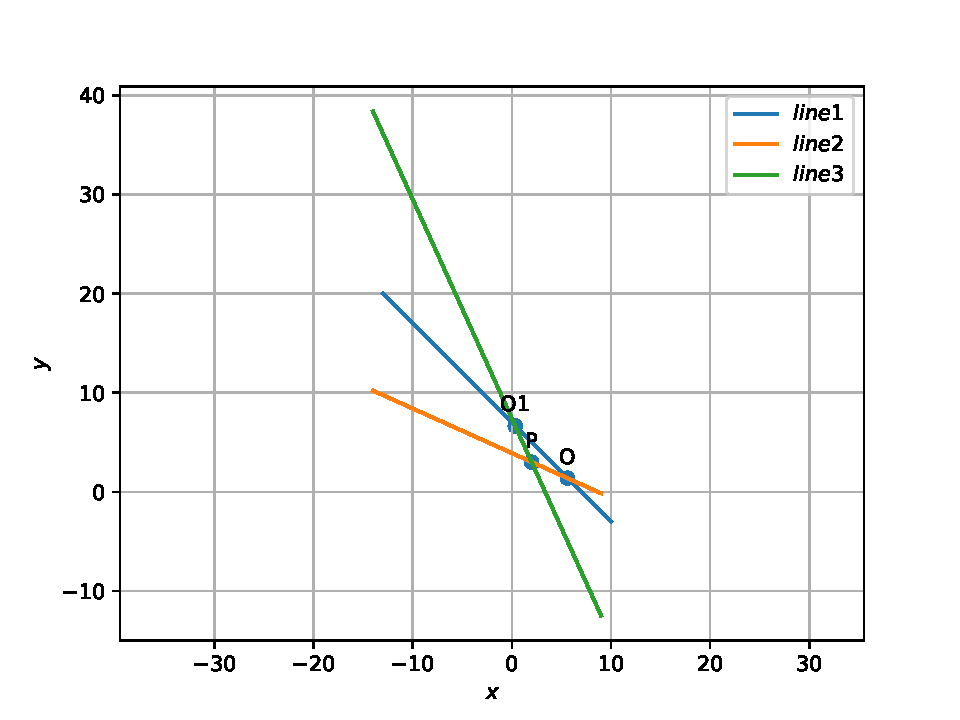
\includegraphics[scale=0.6]{../../python/figs/line1.pdf} 
 \end{center}\vspace{1mm}
 
 \vspace{2mm} \textbf{Construction}
\begin{center}
\setlength{\arrayrulewidth}{0.5mm}
\setlength{\tabcolsep}{6pt}
\renewcommand{\arraystretch}{1.5}
    \begin{tabular}{|l|c|}
    \hline 
    \textbf{vertex} & \textbf{coordinates} \\ \hline
   $\vec{P}$ & $\myvec{
   2\\
   3
   } $ \\ \hline
   d&4\\ \hline
  
      \end{tabular}
  \end{center}
  
\raggedright  Download the code \\
Github link: \href{https://github.com/KrishnaYadati/Assignments/blob/main/Matrix-line_assignment/line_program/line1.py}{Assignment-4}.
  \end{multicols}
\end{document}
